
%%%%%%%%%%%%%%%%%%%%%%% file typeinst.tex %%%%%%%%%%%%%%%%%%%%%%%%%
%
% This is the LaTeX source for the instructions to authors using
% the LaTeX document class 'llncs.cls' for contributions to
% the Lecture Notes in Computer Sciences series.
% http://www.springer.com/lncs       Springer Heidelberg 2006/05/04
%
% It may be used as a template for your own input - copy it
% to a new file with a new name and use it as the basis
% for your article.
%
% NB: the document class 'llncs' has its own and detailed documentation, see
% ftp://ftp.springer.de/data/pubftp/pub/tex/latex/llncs/latex2e/llncsdoc.pdf
%
%%%%%%%%%%%%%%%%%%%%%%%%%%%%%%%%%%%%%%%%%%%%%%%%%%%%%%%%%%%%%%%%%%%


\documentclass[runningheads,a4paper]{llncs}

\usepackage{amssymb}
\setcounter{tocdepth}{3}
\usepackage{graphicx}
\usepackage{float}
\usepackage[full]{complexity}
\usepackage{amsmath}
%\usepackage{amsfonts}
%\usepackage{amsthm}
\usepackage{subfigure}
%\usepackage{caption}
%\usepackage{subcaption}
%\usepackage{cite}
\usepackage{hyperref}
\usepackage{url}
\usepackage{clrscode4e}
\usepackage{verbatim}
\urlstyle{same}
\newcommand{\keywords}[1]{\par\addvspace\baselineskip
\noindent\keywordname\enspace\ignorespaces#1}

% Uniform numbering for previously defined theorem environments (e.g., LNCS).
\makeatletter
\let\c@lemma=\c@theorem
\let\c@corollary=\c@theorem
\let\c@fact=\c@theorem
\makeatother

% Redefinition of LNCS or SODA or Springer proof environment to put a \Box at
% the end of every proof.
\let\realendproof=\endproof
\def\endproof{\hspace*{\fill}$\Box$\realendproof}

\begin{document}

\mainmatter  % start of an individual contribution

% first the title is needed
\title{The Complexity of Determining Critical Sets}

% a short form should be given in case it is too long for the running head
\titlerunning{The Complexity of Determining Critical Sets}

% the name(s) of the author(s) follow(s) next
%
% NB: Chinese authors should write their first names(s) in front of
% their surnames. This ensures that the names appear correctly in
% the running heads and the author index.
%
\author{Fermi Ma \and Ariel Schvartzman \and Erik Waingarten}
%
\authorrunning{Fermi Ma \and Ariel Schvartzman \and Erik Waingarten}
% (feature abused for this document to repeat the title also on left hand pages)

% the affiliations are given next; don't give your e-mail address
% unless you accept that it will be published
\institute{MIT,\\
77 Mass Ave., Cambridge, MA 02139, USA, \\
\protect\url{{fermima,arielsc,eaw}@mit.edu}}

%
% NB: a more complex sample for affiliations and the mapping to the
% corresponding authors can be found in the file "llncs.dem"
% (search for the string "\mainmatter" where a contribution starts).
% "llncs.dem" accompanies the document class "llncs.cls".
%

\maketitle

\section{Introduction}

In 2012, McGuire, Tugermann, and Civario confirmed the conjecture that there are no uniquely solvable 16-clue Sudoku puzzles \cite{mcguire2012there}. It had long been known that 17 clues was sufficient, and there exists an online database containing over 50,000 such puzzles. Thus, the result by McGuire et al. completely solves the problem of determining the minimum number of Sudoku clues needed.

We consider a following generalization of the above Sudoku question: for any given problem, what is the fewest number of clues necessary to make it uniquely solvable? For example, if the problem is to find a Hamiltonian cycle in a given graph $G = (V,E)$, our question would be to determine the minimum number of edges you can specify before only one Hamiltonian cycle contains all of these edges. This general problem is motivated by possible applications to puzzle-making. A puzzle-maker for a newspaper might want to make a puzzle that contains as few clues as possible, but is still uniquely solvable (as the puzzle-maker might want to publish the answer in the next day's paper).

We formalize this problem by defining the ``Fewest Clues Problem" ($\mathsf{FCP}$). We treat $\mathsf{FCP}$ as a new complexity class and we consider the idea of $\mathsf{FCP}$-hard problems. We use this framework to analyze the $\mathsf{FCP}$ versions of classic $\NP$-hard problems such as SAT and 3SAT, as well as $\NP$-hard puzzle problems such as Latin square completion and Sudoku completion. 

The paper is organized as follows. In Section~\ref{sec:related}, we discuss previous research done on this sort of problem for the specific cases of Sudoku, Latin Squares, and graph coloring. We note that while this specific problem has been studied extensively, it is almost always done so with respect to a certain problem. In Section~\ref{sec:prelim}, we motivate and formally define the complexity class $\mathsf{FCP}$. We state what it means for a problem to be $\mathsf{FCP}$, and provide a framework for $\mathsf{FCP}$ reductions. In Section~\ref{sec:The Problems}, we consider $\mathsf{FCP}$ versions of the SAT, 3SAT, Triangle Partition, Latin Squares and Sudoku completion problems, and show why these problems are $\mathsf{FCP}$-hard. Then in Section~\ref{sec:relationship}, we show how the complexity class $\mathsf{FCP}$ fits into the landscape of well-known classes such as $\mathsf{P}, \mathsf{NP}, \Sigma_2^P$, and $\mathsf{PSPACE}$. Finally, in Section~\ref{sec:conclusion} we give concluding remarks and ideas for further research.


\subsubsection{Related Work.}
\label{sec:related}

This problem has been investigated before under a variety of different names. The problem of determining the smallest Sudoku has been referred to as the ``minimum number of clues problem" in
by McGuire et al. in \cite{mcguire2012there}, as well as the ``minimal fair puzzle" problem. The problem of finding the smallest partial Latin Square with a unique solution has been called the ``minimum critical set" problem by Ghandehari et al. in \cite{Ghandehari2005121}. They present upper and lower bounds for this problem. 

In 2013, Cooper and Kirkpatrick \cite{Cooper:2014:CSS:2612293.2612628} extended this problem beyond the realms of puzzles. They introduce a similar notion for the graph coloring problem. Given a graph and a proper coloring of the graph, they refer to a \emph{critical set} as the smallest set of vertices such that when the coloring is restricted to them, there is a unique proper coloring for the rest of the graph. In order to understand the complexity of this problem, they define problems that are natural upper and lower bounds of it. They show that computing the upper and lower bounds is $\NP$-hard. 

To the knowledge of the authors, there aren't any significant efforts to generalize this concept to $\NP$ search problems. 

\section{$\mathsf{FCP}$-: Fewest Clues Problem}
\label{sec:prelim}

\subsection{Formalizing the Question}

In this section, we formalize the question of determining the fewest number of clues for a given instance of a problem. We will be working with $\NP$ search problems, this is the class of problems whose decision is in $\NP$, but we ask for a particular solution. In the case of Hamiltonian Path, instead of asking does there exists a Hamiltonian path, we are asking to present a Hamiltonian path. It is clear that $\NP$ search problems are ``harder" than decision problems, since one can answer the decision problem once one has found a solution.

In particular, we will have an $\NP$ search problem be comprised of a set of \emph{instances}, which will be strings $x$ over some finite alphabet, and for an instance a set of possible \emph{solutions} to be strings $s$ of polynomial size with respect to $|x|$ over some finite alphabet. Each problem also comes with an algorithm $A$ that checks whether a string $s$ is in fact a solution for an instance $x$.

A \emph{clue} will be an indexed character of a solution. So a clue indicates what character lies at some position of the solution.

\begin{definition}
Given some $\NP$ search problem $A$, the ``fewest clues" variation of $A$, $(\mathsf{FCP} A)$ asks for the minimum number of clues corresponding to a unique solution for any given instance.
\end{definition}

This set-up allows us to ask $\mathsf{FCP}$ variations to the common puzzles like Sudoku quiet easily. For the classical $9 \times 9$ Sudoku, we let the alphabet be $\Sigma = \{ 1, ..., 9 \} \cup \{ \Box \}$, and we let an instance be a string of length 81 with elements from $\Sigma$, where each position in the string corresponds to a position on the $9 \times 9$ Sudoku board. The presence of $\Box$ indicates that position is unknown. A solution will be a string of length $81$ with no $\Box$ characters. 

The algorithm $A$ checks whether a solution is correct first checks that in every row, every column, and every $3 \times 3$ square contains all the numbers from $\{1 , ..., 9\}$ and that the solution contains the same numbers as the instance at the specified positions. Figure~\ref{fig:blanksudoku} shows a blank Sudoku puzzle indicating the rows, columns, and $3 \times 3$ squares.

\begin{figure}
\centering
\label{fig:seventeencluesudoku}
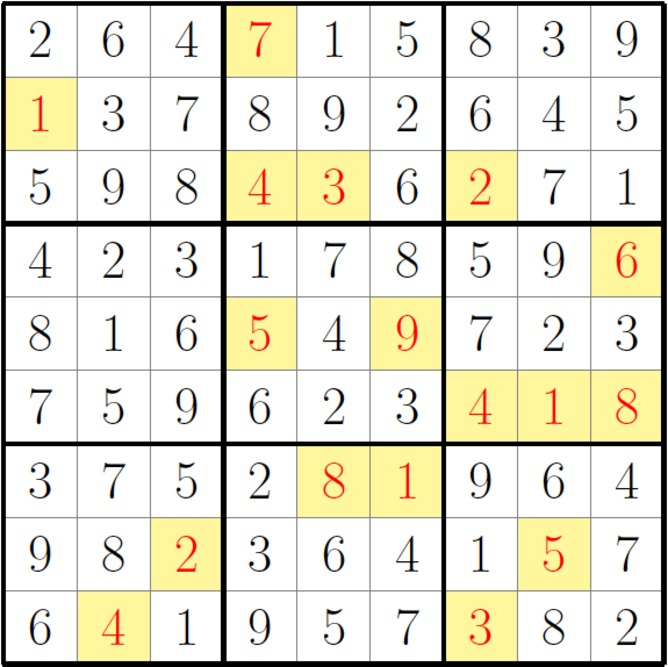
\includegraphics[width=0.5\linewidth]{seventeencluesudoku.jpg}
\caption{17-Clue $9 \times 9$ Sudoku, taken from \cite{smallsudoku}}
\end{figure}

Therefore, the $\mathsf{FCP}$ Sudoku puzzle asks which is the fewest number of squares we must fill in order for the Sudoku to be uniquely solvable. A solution for the $9 \times 9$ case where the instance is initially empty is given in Figure~\ref{fig:seventeencluesudoku}. The fewest clues are given by the yellow squares.

We can also ask the corresponding decision question for some fewest clues problem: does there exist less than $k$ clues which uniquely specify a solution for a given instance? By being able to answer this question, we can solve for the minimum number of clues necessary with a binary search through $k$.

\subsection{The $\mathsf{FCP}$ Class}

We now present definitions that give rise to a complexity class, which we call  $\mathsf{FCP}$ (Fewest Clues Problem). This will sound very familiar to the above notions of solution and clue. We generalize the $\mathsf{FCP}$ variation to all $\NP$ search problems without having to explicitly specify the instance, solution and checker algorithm by framing the problem in terms of non-deterministic Turing machines. This generalization will give us an easy extension of the Cook-Levin theorem, which will show that $\mathsf{FCP}$ SAT is $\mathsf{FCP}$-complete.

We can assume without loss of generality that non-deterministic Turing machines (NTMs) have a branching factor of $2$ at each non-deterministic step. In addition, when the NTM performs a non-deterministic step where the computation branches, we assume that we have a canonical ordering of the two branches. We can call one the ``left" branch, and the other the ``right" branch. We also assume without loss of generality that all branches of the computation have length equal to a fixed polynomial since we are only dealing with $\NP$- search problems.

\begin{definition}
A partial certificate is a read-only tape which contains at each tape cell one of three possible characters, 0, 1, or $\bot$.
\end{definition}

\begin{definition}
The size of a partial certificate is the number of non-null entries. 
\end{definition}

For any $\NP$ search problem, a partial certificate is the generalization of a certificate. Also, any certificate of an $\NP$ problem can be thought of as a partial certificate. We think of partial certificates as ordinary certificates with some tape cells erased.

\begin{definition}
A modified non-deterministic Turing machine (mNTM) is an NTM where there is an additional input of a partial certificate. At each step of the computation, an mNTM reads the next tape cell of the partial certificate and if the partial certificate contains a 0, it takes the left branch of the computation. If it contains a 1, it takes the right branch of the computation. If it contains $\bot$, then it behaves non-deterministically. Other than that, an mNTM behaves exactly like an NTM.
\end{definition}

In some sense, a partial certificate makes an mNTM more deterministic. If a partial certificate contains no $\bot$ characters, then the mNTM behaves like a deterministic Turing machine. Alternatively, we can think of the partial certificate as feeding in clues to the mNTM in order to guide its computation. It is clear that given any NTM, we can construct a corresponding mNTM which runs in exactly the same manner, but has an additional input of a partial certificate. With these definitions, we are ready to define the class $\mathsf{FCP}$.

\begin{definition}
$\mathsf{FCP}$ is the class of function problems of the following form:
\begin{quote}
Given an NTM running in polynomial time along with an input $x$, compute the smallest a partial certificate such that the corresponding mNTM running on $x$ with the partial certificate has only one accepting branch?
\end{quote}
\end{definition}

\begin{proposition}
Any problem in $\mathsf{FCP}$ can be phrased as a fewest clues problem.
\end{proposition}

\begin{proof}
Suppose we are given NTM $M$ which runs in polynomial time with respect to the length of the input. We create a fewest clues problem $\mathsf{FCP} M$:
\begin{itemize}
\item Instances: these are the instances of the NTM
\item Solutions: these are strings with characters in $\Sigma = \{ 0, 1 \}$.
\item Checker algorithm: Given an instance $x$ and a solution $s$, simulate an mNTM which corresponds to the NTM $M$ with partial certificate $s$. If the runtime of the mNTM is not equal to $|s|$, then reject. If it is equal, and so the mNTM behaves deterministically and accepts, then accept. 
\end{itemize}
\begin{enumerate}
\item Each clue in $\mathsf{FCP} M$ corresponds to a character in the certificate.\\
Proof: This is because each clue is an indexed character of the solution, which is in turn an indexed character of a certificate.
\item A set of clues corresponds to a partial certificate for $M$.\\
Proof: This follows from $1$ by taking many of characters in the certificate.
\item If $C$ is a set of clues with a unique solution, then the corresponding partial certificate will have a unique accepting branch.\\
Proof: Suppose there is another accepting branch in the mNTM. The non-deterministic turns at each step specify two possible solutions for the set of clues $C$. 
\item If $C$ is the smallest set of clues with a unique solution, then the corresponding partial certificate is the smallest partial certificate with mNTM having a unique accepting branch.\\
Proof: Follows from 3 and the fact that the size of the partial certificate is the same as the number of clues.
\item Therefore, a problem in $\mathsf{FCP}$ can be phrased as a fewest clues problem.\\
Proof: follows from $4$ and because each partial certificate corresponds to a set of clues.
\end{enumerate}
\end{proof}

\begin{proposition}
Any fewest clues problem with solution alphabet $\Sigma = \{ 0 ,1 \}$ is in $\mathsf{FCP}$.
\end{proposition}

\begin{proof}
We assume that we have some fewest clues problem, $\mathsf{FCP} A$, where:
\begin{itemize}
\item The set of instances is $I$.
\item The set of solutions is $S(x)$ for each $x \in I$ where each string is a character from some alphabet $\Sigma$ and each $s \in S(x)$ has $|s| \leq p(|x|)$.
\item We have an algorithm $A$ with inputs $x \in I$, $s \in S$ that decides in polynomial time whether $s$ is a solution to $x$.
\end{itemize}
We will construct a NTM $M$ such that the smallest partial certificate for $M$ will correspond to the fewest clues in $\mathsf{FCP} A$. \\
NTM $M$: Given an instance $x$, non-deterministically, for $p(|x|)$ steps, generate a solution $s$ by writing a character in each step, where the left branch writes $0$ in the solution and the right branch writes $1$ in the solution. Then simulate $A$ with inputs $x$ and $s$. Accept if $A$ accepts, and reject if $A$ rejects. 
\begin{enumerate}
\item A partial certificate corresponds to a set of clues of the same size.\\
Proof: The partial certificate only applies to non-deterministic steps, where $M$ writes down a solution. Therefore, a partial certificate tells the mNTM which characters to write at which positions deterministically, which correspond to a set of clues.
\item If a partial certificate has an mNTM with only one accepting branch, then the corresponding set of clues has a unique solution.\\
Proof: If the partial certificate has only one accepting branch, then it means that the corresponding set of clues have only a unique way to complete the clues to have a solution, since each branch explores every possible solution which is a superset of the set of clues.
\item If there exists a set of clues with a unique solution, there exists a partial certificate with only one accepting branch.\\
Proof: The set of clues specifies a partial certificate. If there is one way to fill the set of clues to have a solution, each solution will correspond to a branch of the computation. 
\item The smallest partial certificate with a unique accepting branch in the mNTM is the smallest set of clues with a unique solution.\\
Proof: follows from 2 and 3 and the fact that corresponding partial certificates and sets of clues have the same size. 
\end{enumerate}
\end{proof}

We are almost there, we just need to show that the condition that $\Sigma = \{ 0, 1\}$ is unnecessary. We do this by cleverly choosing how to branch.

\begin{proposition}
Any fewest clues problem is in $\mathsf{FCP}$.
\end{proposition}

\begin{proof}
The only problem with the above proof for arbitrary \emph{finite} $\Sigma$ is that we simply cannot write down every possible solution in the non-deterministic step in $p(|x|)$ steps. Let $|\Sigma| = \sigma$. If we require the NTM $M$ to have branching factor $2$, it will take at least $\log \sigma$ non-deterministic steps to specify a unique character in $\Sigma$ to write down. This is a problem, since a specific character in the partial certificate might not be a clue, but rather might say, ``the $i$th character of the solution is in the first half of $\Sigma$". We would no longer maintain the number of clues equal to the size of the partial certificate, since each clue would correspond to $\log \sigma$ characters in a partial certificate.

Instead of taking $\log \sigma$ steps to decide which character of $\Sigma$ to write in the solution, we use $\sigma$ steps. The first non-deterministic step will choose whether to write the first element of $\Sigma$. The second will choose whether to write the second. The third step will choose the third element of $\Sigma$ and so on (see Figure~\ref{fig:branching}). Since each branch of the computation must be the same length, once we pick, we continue branching for $\sigma$ steps, and if we ever take a right branch again, will reject. I claim now that each partial certificate corresponds to a clue of the same size and vice-versa, allowing up to complete the theorem.
\begin{enumerate}
\item Each clue corresponds to a segment of $\sigma$ characters in a certificate.\\
Proof: This is obvious, since it takes us $\sigma$ non-deterministic steps to make a choice of character.
\item There are no 0's in the smallest partial certificate with a unique accepting branch.\\
Proof: Suppose there was a 0 in the smallest partial certificate with a unique accepting branch, then that 0 corresponds to a taking some left branch. The left branch was in the process of picking some character, and suppose the unique accepting branch picked $a \in \Sigma$, then replace the 0 in the partial certificate, with the $1$ which picked $a$ in that segment of $\sigma$ branches. This is also a partial certificate of the same size. 
\item The 1's in the smallest partial certificate are inside their chunk of $\sigma$ branches.\\
Proof: if there were two 1's inside the chunk, the branch will reject.
\item If the $i$th branch of the $j$th chunk of $\sigma$ branches in the smallest partial certificate corresponds to the clue of picking the $i$th element of $\Sigma$ for index $j$ in the solution.\\
Proof: follows from the fact that there are only 1's, each in their $\sigma$ long chunks.
\item Each smallest partial certificate with unique accepting branch corresponds to a set of clues of the same size with a unique solution. \\
Proof: this follows from 4 and the fact that we know how to go from clues to partial certificates.
\end{enumerate}
\end{proof}

\begin{figure}
\centering
\label{fig:branching}
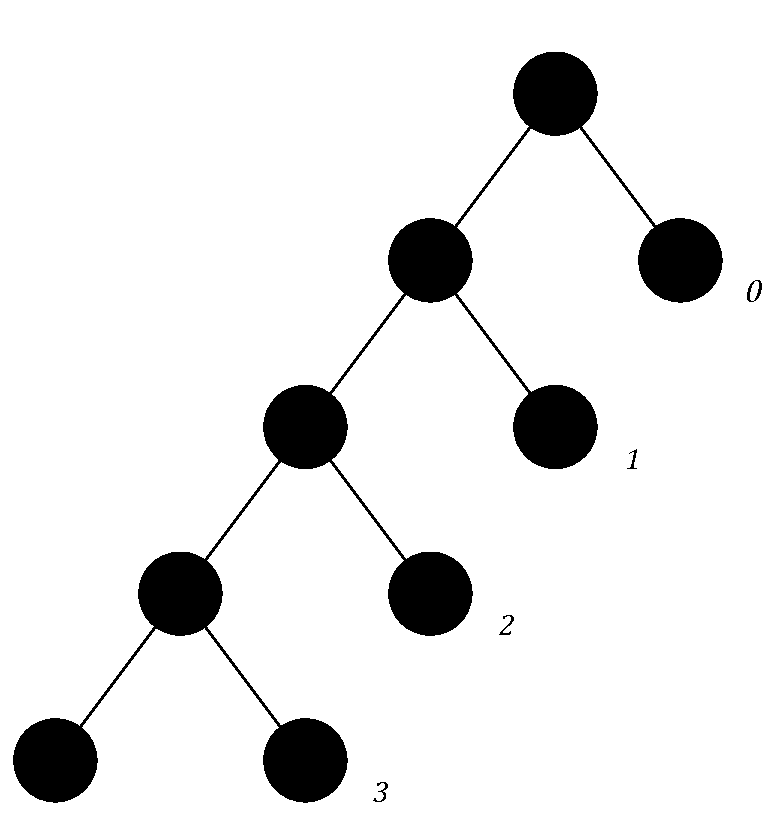
\includegraphics[width=0.4\linewidth]{branching.pdf}
\caption{Branching to pick $\Sigma = \{ 0, 1, 2, 3 \}$}
\end{figure}

The above proposition justifies our analysis of this class for answering these questions.

\section{Some $\mathsf{FCP}$-complete Problems.}
\label{sec:The Problems}

In this section, we proceed to show that $\mathsf{FCP}$ Sudoku is $\mathsf{FCP}$-complete. In order to do so, we first show that $\mathsf{FCP}$ SAT is $\mathsf{FCP}$-complete. We then follow a known chain of reductions that is used to show that the problem of filling in a Sudoku is $\NP$-complete. 

\subsection{$\mathsf{FCP}$ SAT}
The following is the fewest clues version of the Boolean satisfiability problem.

\begin{itemize}
\item Instance: a Boolean formula $\phi$.
\item Question: What is the smallest partial assignment of the variables which is uniquely satisfiable?
\end{itemize}

We will prove that $\mathsf{FCP}$ SAT is $\mathsf{FCP}$-complete using the same construction as in the Cook-Levin theorem. We include the theorem here since our proof draws on many of their ideas. The proof is from \cite{Garey}, but the authors give it as it appears in Wikipedia.

\begin{theorem}
\label{thm:cooklevin}
SAT is $\NP$-complete.
\end{theorem}

\begin{proof}
For any NTM $M$ which runs in polynomial time, and given an input $x$ to the $M$, we will make a Boolean expression $\phi$ of polynomial size in $x$ such that the formula is satisfiable if and only if $M$ accepts on input $x$. 

Recall that a NTM $M$ is defined by a tuple of states $Q$, $\Sigma$ a finite alphabet of tape symbols, $s \in Q$ a starting state, $F \subset Q$ a set of accept states, and $\delta \subset ((Q - F) \times \Sigma) \times (Q \times \Sigma \times \{ -1, 1\}))$ is the non-deterministic transition function. Suppose $M$ runs in $p(|x|)$ where $p$ is some polynomial.

For each $q \in Q$, $-p(|x|) \leq i \leq p(|x|)$, $j \in \Sigma$, and $0 \leq k \leq p(|x|)$, we have the variables outlined in the following table:\\
\begin{center}
\begin{tabular}{| l | l | l |}
  \hline    
  Variables & Intended Interpretation & How many?\\
  \hline \hline          
  $T_{i,j,k}$ & True if the tape cell $i$ contains the symbol $j$ at time $k$ & $O(p(|x|)^2)$ \\
\hline
  $H_{i,k}$ & True if the head position is at tape cell $i$ at time $k$ & $O(p(|x|)^2)$ \\
\hline
  $Q_{q, k}$ & True if the NTM is at state $q$ at time $k$ & $O(p(|x|))$ \\
  \hline  
\end{tabular}
\end{center}
Now that we've defined polynomially many variables, we will make the clauses of the Boolean formula.
\begin{center}
\begin{tabular}{| l | l | l | l |}
  \hline    
  Clause & Conditions & Interpretation & How many?\\
  \hline \hline
  $T_{i,j,0}$ & \begin{tabular}{l} Cell $i$ contains \\ $j\in \Sigma$ initially \end{tabular} & initial content of tape match $x$ & $O(p(|x|))$ \\
\hline
  $Q_{s, 0}$ & & set starting state & 1 \\
\hline
  $H_{0,0}$ & & starting head position at 0 & 1 \\
\hline
  $\neg T_{i,j,k} \vee \neg T_{i,j', k}$ & $j \neq j'$ & at most one symbol per cell & $O(p(|x|)^2)$\\
\hline
 $\bigvee_{j \in \Sigma} T_{i,j,k}$ & & at least one symbol per cell & $O(p(|x|)^2)$ \\
\hline
 $T_{i,j,k} \wedge T_{i,j',k+1}\rightarrow H_{i,k}$ & $j \neq j'$ & tape only changes when written & $O(p(|x|)^2)$ \\
\hline
 $\neg Q_{q, k} \vee \neg Q_{q', k}$ & $q \neq q'$ & Only one state at a time & $O(p(|x|))$ \\
\hline
 $\neg H_{i,k} \vee \neg H_{i', k}$ & $i \neq i'$ & Only one head position at a time & $O(p(|x|)^2)$ \\
\hline
$\begin{array}{l}
(H_{i,k} \wedge Q_{q,k} \wedge T_{i,\sigma,k}) \rightarrow \\
\bigvee_{(q, \sigma, q', \sigma',d) \in \delta} \\ (H_{i+d, k+1} \wedge Q_{q', k+1} \wedge T_{i,\sigma',k+1}) \end{array}$ & $k \leq p(|x|)$ & possible transitions & $O(p(|x|)^2)$\\
  \hline  
$\bigvee_{k \leq p(|x|)} \bigvee_{t\in F} Q_{f,k}$ & & must have an accepting state & 1 \\
\hline
\end{tabular}
\end{center}
If the formula is satisfiable, then the satisfying assignments corresponds to a branch of the computation on $M$. Likewise, if there is an accepting branch, then the computation through that branch given the values of the variables, since the branch is accepting, all the clauses are satisfied.
\end{proof}

\begin{theorem}
\label{thm:cooklevinanalog}
$\mathsf{FCP}$ \text{SAT} is $\mathsf{FCP}$-complete.
\end{theorem}

\begin{proof}
We use the reduction from the Cook-Levin theorem, described in Theomem~\ref{thm:cooklevin}.

\begin{enumerate}
\item We assume that we have a NTM $M$ with input $x$ running in polynomial time.
\item We compute the Boolean formula $\phi$ corresponding to $M$ with input $x$ as in the Cook-Levin theorem.
\item Since we assumed that $M$ has branching factor at most $2$, at each step, we add the variables $l_k$ which is True if and only if $M$ takes the left branch of the computation at time $k$.
\item We transoform each clause $(H_{i,k} \wedge Q_{q,k} \wedge T_{i, \sigma, k}) \rightarrow \bigvee (H_{i+d,k+1} \wedge Q_{q',k+1} \wedge T_{i,\sigma',k+1})$ into 
\[
 (H_{i,k} \wedge Q_{q,k} \wedge T_{i,\sigma, k}) \rightarrow \left(\begin{array}{c} (H_{i+d,k+1} \wedge Q_{q', k+1} \wedge T_{i,\sigma', k+1} \wedge l_k) \\ \vee \\ (H_{i+d',k+1} \wedge Q_{q'', k+1} \wedge T_{i,\sigma'', k+1} \wedge \neg l_k) \end{array}\right) \]
Proof: Here, we are encoding in the variable $l_k$, whether we took the left branch or the right branch. Also, we are using the fact that the non-deterministic transition contains only two possible branches.
\item We add the following clauses to obtain $\phi'$:
\[ (H_{i,k} \wedge Q_{q,k} \wedge T_{i,\sigma,k} \wedge l_k) \leftrightarrow a_{l, i, q, \sigma, k} \]
\[ (H_{i,k} \wedge Q_{q,k} \wedge T_{i,\sigma,k} \wedge \neg l_k) \leftrightarrow a_{\neg l, i, q, \sigma, k} \]
Proof: We can do this without increasing $\phi$ too much since we have $O(p(|x|)^2)$ clauses.
\item $\phi'$ is satisfiable if and only if $\phi$ is satisfiable. \\
Proof: We know whenever $\phi'$ is satisfiable, $\phi$ is satisfiable since it contains more clause requirements. Now if $\phi$ is satisfiable, then we know that for each time $k$, only one of each head, state, and time position variables are True, in addition, we either took the left branch, or right branch, so that gives us the value of $l_k$, so we set the corresponding $a_{l, i,q,\sigma,k}$ or $a_{\neg l, i, q, \sigma, k}$ to True and all other $a_{l, i', q', \sigma', k}$ and $a_{\neg l, i', q', \sigma', k}$ to False.
\item Let $P$ be the smallest partial assignment of the variables in $\phi'$ such that $\phi'$ is uniquely satisfiable after the assignment.
\item In order to simplify notation, we use $l'$ be the literal $l$ or $\neg l$.
\item Suppose some $a_{l', i, q, \sigma, k}$ in $P$ is assigned to False, then we can replace it with some other $a_{l'', i', q', \sigma', k}$ which is assigned to True. \\
Proof: In the unique solution, there is some $a_{l', i', q', \sigma', k}$ which is True. We also know that $a_{l'', i',q',\sigma',k} \rightarrow \neg a_{l',i, q, \sigma, k}$ since there can only be one state variable, one head position variable, and one tape cell variable for that head position be True at that time. 
\item We can find this is alternate $a_{l'', i', q', \sigma', k}$ in polynomial time.\\
Proof: There are polynomially many $a_{l'', i',q',\sigma',k}$ so we can write the formula $\phi'$ which remains after all the $P - \{a_{l', i, q, \sigma, k}\}$ are assigned. Furthermore, we assign $a_{l'', i', q',\sigma', k}$ and check whether the smallest partial assignment of this formula is empty (i.e. there exists a unique solution).
\item Likewise, if there is any other type of variable in $P$ which is assigned to False, we can replace it with a True variable.\\
Proof: the same procedure works as in $6$ and $7$ work.
\item If some variable in $P$ is not a variable of type $a$, then we can replace it by a variable of type $a$.\\
Proof: Existance holds since at that step, there is an action taken by NTM $M$, and we can find it by the same procedure as in $7$. 
\item So we can find a smallest partial assignment $P$ made up of all variables of the form 
\[ a_{l', i,q,\sigma, k} \]
Proof: follows from $7$ and $9$.
\item The variables $a_{l', i,q,\sigma, k}$ being True, indicate whether at a given time, $M$ took a left branch or a right branch.\\
Proof: In fact, we have complete information of the transition NTM $M$ made at the $k$th step. If $l' = l$, then we took a left branch, if $l' = \neg l$, then we took a right branch.
\item If the partial assignment has a unique satisfying assignment, then the mNTM $M$ has a unique accepting branch. \\
Proof: This follows from $14$ and the fact that each assignment of the variables corresponds bijectively with a branch of the computation of $M$. 
\item The smallest partial assignment with a unique satisfying assignment is the same size as the smallest partial certificate with a unique accepting branch.\\
Proof: For each variable, we have one indication of a branch, and for each transition made by an accepting branch, we have a variable in the partial certificate. 
\end{enumerate}

\end{proof}

%%%%
%%%% Thought of a better proof
%%%%
\begin{comment}
\item We make NTM $M'$ with alphabet $\Sigma \times Q$, and whenever $M$ is in state $q$ and will write $\sigma$ on the tape, $M'$ writes $(\sigma, q)$. \\
Proof: Note that we can do this without increasing the runtime or the description of the NTM significantly. Each branch of the computation of $M'$ corresponds bijectively with a branch in $M$.
\item We use the Cook-Levin reduction to get a Boolean formula $\phi$ corresponding to that $M'$ with input $x$. \\
Proof: $\phi$ is still polynomial in the size of $M$ and $x$. 
\item Let $\Phi$ be a partial assignment of the variables in $\phi$. 
\item Suppose some variable $a$ in $\Phi$ is assigned to False.\\
There are three possible cases to check:
\begin{itemize}
\item $a = T_{i,j,k}$: In this case, then by the clause $\bigvee_{j' \in \Sigma} T_{i,j',k}$ means one of $T_{i,j',k}$ is True, and by clause $\neg T_{i,j,k} \vee \neg T_{i,j',k}$, we can replace $a$ with $T_{i,j',k}$ assigned to True.
\item $a = H_{i,k}$: In this case, then by the transition clause $(H_{i,k} \wedge Q_{q,k} \wedge T_{i,\sigma,k}) \rightarrow \bigvee (H_{i+d,k+1} \wedge Q_{q',k+1} \wedge T_{i,\sigma', k+1})$ and $H_{0,0}$, one of $H_{i', k}$ must be set to True, and by clause $\neg H_{i,k} \vee \neg H_{i', k}$, we can replace $a$ with $H_{i',k}$ assigned to True.
\item $a = Q_{a,k}$: This is almost the exact same argument as the case for head position variables, since we have exactly one state be True at each time step.
\end{itemize}
\item So we can replace a variable assigned to False into a variable assigned to True in polynomial time.\\
Proof: There are polynomially many variables, and we can switch one at a time in polynomial time as shown in 5.
\item Suppose $a \in \Phi$ is a state variable $Q_{q,k}$ set to True, then we can replace $a$ with some tape variable $T_{i,j,k}$ which is set to True.\\
Proof: We know that some tape variable was written at time $k$, which contained the value of $Q_{q,k}$, therefore, 
\end{enumerate}
%%%
%%% End of draft proof
%%%
\end{proof}

\begin{proof}
We use  proof is similar to that of the Cook-Levin theorem presented in \cite{Garey}. We first turn an arbitrary NTM into an NTM with a bigger alphabet where at each step, if the NTM in state $q$ writes $a$ into some tape cell, then the other NTM writes $(q,a)$ into the same tape cell. Once we have this, we apply the reduction from the Cook-Levin theorem to get a Boolean formula $\phi$. 

We claim that if $\phi$ has a partial assignment of $k$ variables with a unique complete assignment, then there exists a partial certificate for the NTM with corresponding mNTM having only one accepting branch of the computation.

Note that if a partial assignment of $k$ variables contains a variable that is set to false, then the variable is a head position variable, a state variable, or a tape cell variable. We know that there exists a head position variable, a state variable, and a tape cell variable which is true at each time, so if we switch the corresponding variables, we have removed a false variable, added a true variable. By analyzing $\phi$, the true variable implies that the false variable is false, therefore, we still have a partial certificate. 

This implies that we can assume that all assignments are true. If we have a head position variable, the tape cell variable at that given position will be set to true, and so switching them will maintain the partial assignment. Also, since the content of each tape cell is the state-content tuple, a state variable can be replaced by the tape cell variable.

Since each complete assignment of the variables corresponds to a unique accepting branch of the computation, knowing the contents of the tape cell at each time tells you which branch of the computation to take. Therefore, if there exists a partial assignment of $k$ variables which yield a unique complete assignment, then there exists a partial certificate of size $k$ whose mNTM has a unique accepting branch.
\end{proof}
\end{comment}

From this we can easily show that the fewest clues version of the 3SAT problem is $\mathsf{FCP}$-complete.

\begin{theorem}
\label{thm:3sat}
$\mathsf{FCP}$ 3SAT is $\mathsf{FCP}$-complete.
\end{theorem}

\begin{proof}
We reduce from $\mathsf{FCP}$ SAT. 
\begin{enumerate}
\item We assume without loss of generality that each SAT formula is a conjuction of clauses, where each are disjunctions.\\
Proof: these are the kind of Boolean formulas we get from the Cook-Levin theorem.
\item Suppose $C$ is a clause, we define a function $g$ to handle $C$. There are four cases:
\begin{itemize}
\item $C = x_1$. Then we let $g(C) = (x_1 \vee x_1 \vee x_1)$.
\item $C = (x_1 \vee x_2)$. Then we let $g(C) = (x_1 \vee x_2 \vee x_1)$.
\item $C = (x_1 \vee x_2 \vee x_3$), then we just let $g(C) = C$. 
\item $C = (x_1 \vee x_2 \vee \dots \vee x_n)$, then we let
\[ g(C) = (x_1 \vee x_2 \vee z_2) \wedge (\overline{x_2} \vee \overline{z_2}) \wedge (x_2 \vee z_2) \wedge g((\overline{z_2} \vee x_3 \vee \dots \vee x_n)) \]
\end{itemize}
\item $\phi = \bigvee C_i$ is satisfiable if and only iff $\phi' = \bigvee g(C_i)$ is satisfiable.\\
Proof: A satisfying assignment for one gives a satisfying assignment for the other. The only case to check is the last case with big clauses. In this case, we let $z_i = \overline{x_i}$, and this gives a satisfying assignment.
\item If some $z_i$ is in a partial assignment of $\phi'$, we can replace it with a variable $x_i$. \\
Proof: this is because $z_i \leftrightarrow \overline{x_i}$. 
\item There exists a smallest partial assignment of $\phi'$ which contains only variables of $\phi$, and we can find it in polynomial time. \\
Proof: we can replace the added variables using the implication.
\item the smallest partial assignment of $\phi'$ with a unique satifying assignment containing no added variable is a smallest partial assignment of $\phi$ with a unique satisfying assignment. \\
Proof: If $\phi'$ yields a unique satisfying assignment, then so does $\phi$. The only thing to check is that it could not be smaller. This is true because a partial assignment of $\phi$ is a partial assignment of $\phi'$ with the same information. 
\end{enumerate}
\end{proof}

\subsection{Reductions}

By analyzing the previous two reductions (Theorem~\ref{thm:cooklevinanalog} and Theorem~\ref{thm:3sat}), we can generalize the process we used in order to show these problems were $\mathsf{FCP}$-hard. In particular, we started with some $\mathsf{FCP}$-hard problem $\mathsf{FCP} A$, and wanted to show that problem $\mathsf{FCP} B$ was $\mathsf{FCP}$-hard. 

\begin{comment}
We did the following steps:
\begin{enumerate}
\item We defined $f: A \rightarrow B$ which mapped some instances of $A$ into instances of $B$.
\item We identified some special types of clues for $\mathsf{FCP} B$ which corresponded with sets of clues of $\mathsf{FCP} A$. For example, in Theorem~\ref{thm:cooklevinanalog}, we had partial assignments on variables $a_{l', i, q, \sigma, k}$ correspond to actions in the computation. In Theorem~\ref{thm:3sat}, we had assignments on the variables of $x_i$ in $\phi'$ only correspond to assignments on those same variables in $\phi$. 
\item We wanted the correspondence to always keep the same number of clues.
\item We gave a polynomial time algorithm which took any set of clues in $B$ into a set of clues of the identified type of the same size.
\end{enumerate}
This means that if we wanted to solve $\mathsf{FCP} A$ on instance $x$, then we run $\mathsf{FCP} B$ on instance $f(x)$, and given the set of clues $C$, we convert the set of clues into a nice type of clues $C'$ in polynomial time, and then use the correspondence to give a set of clues for $\mathsf{FCP} A$. 
\end{comment}

We summarize our method of reduction in the following lemma.
\begin{lemma}
Let $\mathsf{FCP} A$ be an $\mathsf{FCP}$-hard problem. Let $\mathsf{FCP} B$ be a problem. Denote $C_A$ as the clues of problem $A$ and $C_B$ as the clues for $B$.
\begin{itemize} 
\item Let $f: A \rightarrow B$ map instances of $A$ into instances of $B$. 
\item Let $C_B' \subset C_B$ be a particular set of clues for $C_B$, and $h:C_B' \rightarrow C_A$ be a bijection on the clues.
\item Let $M$ be an algorithm which runs in polynomial time and takes a set of clues for $B$ and outputs a set of clues with clues in $C_B'$ of the same size. 
\end{itemize}
Suppose we satisfy the condition that if $C_{f(x)} \in C_B'$ is a set of clues for $f(x)$, then $\{ h(c) | c \in C_{f(x)}\}$ is a set of clues solution for $x$. Then $\mathsf{FCP} B$ is $\mathsf{FCP}$-hard. 
\end{lemma}

\begin{proof}
Let $x$ be an instance of $\mathsf{FCP} A$. Suppose $C$ is a set of fewest clues of $f(x)$. Then let $M(C) = C_{f(x)}$ is another set of fewest clues with all clues are in $C_B'$. Now I claim that $C_x = \{ h(c) | c \in C_{f(x)}\}$ is a fewest clues set for $x$. We know that its is a set of clues for $x$ by the hypothesis. Suppose that there existed a smaller one, since $h$ is a bijection, it would give us a smaller set of clues for $f(x)$, which would contradict $C_{f(x)}$. 

Suppose that $C_x$ did not yield a unique solution, then there exists $C_{x}^{(1)}, C_x^{(2)}$ such that these sets are not equal, and $C_x \subset C_{x}^{(1)} \cap C_x^{(2)}$ which are clues for different solutions. This would imply that $C_{f(x)}$ has distinct supersets which are subsets of two different solutions.
\end{proof}

As an example, in Theorem~\ref{thm:3sat}, $f: SAT \rightarrow 3SAT$, was the mapping which applied the mapping $g$ to each clause. $C_B'$ was the set of assignments of $\phi'$ whose variables are $x_i$, and $h$ was the identity. The algorithm $M$ took each assignment of $z_i$ and replaced it with an assignment of $x_i$. The algorithm was correct since $z_i \leftrightarrow \overline{x_i}$.

\begin{lemma}
$\mathsf{FCP}$ 1-in-3SAT is $\mathsf{FCP}$-hard. 
\end{lemma}

\begin{proof}
We use the following reduction. We map each clause of $\phi$, $(x_1, x_2, x_3)$ into five clauses,
\[ \begin{array}{c} 
(\overline{x_1}, a, b) \\
(x_2, b, c) \\
(\overline{x_3}, c, d) \\
(b, \overline{f}, f) 
\end{array} \]
Where we added the variables $a, b, c, d, e, f$ for each clause. 
In this case, we pick our special clues to be the clues with variables corresponding to variables in $\phi$. 

Note that in a fewest clues assignment, if any of $a,c,d,f, g, h$ is present, it is present with a value of true. If it is in the fewest clues assignment as a value of false, then if we can derive the truth value of the clause, it would imply the false assignment, so we would get rid of it. 

One issue is that happens if $b$ and $c$ imply the values of two variables. However, if $b$ or $c$ is true, then we must need another clue for $e$ or $f$ (in $b$'s case), or $g$ or $h$ (in $c$'s case). So if $b$ or $c$ is true, we know that two variables are true, 
\end{proof}

\subsection{$\mathsf{FCP}$ Triangle Partition}

This problem is a known $\NP$-complete problem which asks to partition the edges of a graph into triangles \cite{holyer1981np}. We present the fewest clues version of the problem since we will use it to show hardness results for $\mathsf{FCP}$ Latin Squares and $\mathsf{FCP}$ Sudoku. There is a general description of the problem in \cite{holyer1981np}. A specific instance is addressed in \cite{colbourn1984complexity}. We will use the definition in \cite{colbourn1984complexity}. We first present a definition of a property of tripartite graphs which will simplify the analysis.

\begin{definition}
A tripartite graph is \emph{uniform} if each vertex has equally many neighbors in each of the other two partitions.
\end{definition}

\begin{itemize}
\item Instance: A uniform tripartite graph, along with a parameter $k$.
\item Question: Does there exist a set of $k$ triangles such that including them implies a unique partition of the remainder of the graph?
\end{itemize}

Note that if a tripartite graph has a triangle partition, the graph must be uniform. Therefore, we assume without loss of generality that this is the case. 

The following proof is a sketch and is under revision.

\begin{theorem}
$\mathsf{FCP}$ Triangle Partition is $\mathsf{FCP}$-complete.
\end{theorem}

\begin{proof}
We use the reduction from \cite{holyer1981np}, applying the slight modifications made in \cite{colbourn1984complexity} so that the graph is tripartite, additionally we apply another modification which makes us reduce the problem from 1-in-3SAT. We refer the reader to \cite{holyer1981np}, \cite{colbourn1984complexity} for questions about notation.

We define $f$ to map instances to instances. Do the same reduction as in \cite{holyer1981np}, but we make some additional associations. In particular, if variable $x$ appears in clause $c$ as $x$, then \cite{holyer1981np} associates an $F$-patch in $x$ to an $F$-patch in $c_1$. Additionally, we associate a $T$-patch in $x$ to a $T$-patch in $c_1$. By associating $F$-patches, we guarantee that one of $x$ and $c_1$ must be a $T$-partition. By adding the association between a $T$-patch in $x$ and a $T$-patch in $c_1$, we guarantee that one must be an $F$-partition. This means that if $x$ is a $T$-partition, then $c_1$ is an $F$-partition, and if $x$ is an $F$-partition, then $c_1$ is a $T$-partition.

We pick the center triangle of an $F$-patch and a center triangle of a $T$-patch in each variable gadget. This will comprise the special clues for Triangle Partition. The mapping $h$ will be the following. The center triangle of an $F$-patch of a variable will map to assigning that variable to true. The center triangle of a $T$-patch of a variable will map to assign that variable to false. 

Now we give the algorithm $M$. Note that if you know any triangle in the partition, then that triangle necesarily implies a partition in that graph, which will be connected to a partition in a variable, which means we can replace that triangle, with our special triangle in the variable. So algorithm $M$ determines the partition of the clause gadget or the variable gadget and using the fact that an partitions of clauses connect to partitions of variables, we can replace the arbritrary triangles in the clues with the special triangles in the variables. 

Since clues for Triangle Partition map to clues of 1-in-3SAT, $\mathsf{FCP}$ Triangle Partition is $\mathsf{FCP}$-hard.
\end{proof}

\subsection{$\mathsf{FCP}$ LatinSquares}

In Latin Squares we are given a $n \times n$ grid, some of whose entries have been filled in with numbers from $1$ to $n$. The goal of the game is to fill the rest of the grid with numbers from $1$ to $n$ while enforcing that no row or column repeats a number. 

It is known that such problem is $\NP$-complete. We present the problem $\mathsf{FCP}$ Latin Squares in our framework.

\begin{itemize}
\item Instance: A partially filled latin square, along with a parameter $k$. 
\item Question: Does there exists set of at most $k$ entries such that pre-setting them implies a unique solution?
\end{itemize}


\begin{theorem}
$\mathsf{FCP}$ Latin Squares is $\mathsf{FCP}$-complete.
\end{theorem}

\begin{proof}
We do this via reduction from $\mathsf{FCP}$ TrianglePartition. Given a tripartite graph $G$, we first check whether or not it is uniform. If it is not uniform, then there does not exist a triangle partition. If it is uniform, we can write down a Latin framework $LF(G;2n,2n,2n)$ in polynomial time \cite{colbourn1984complexity}. Since the Latin framework is constructed so that $G$ is the defect of $LF(G;2n,2n,2n)$, there is a triangle partition of $G$ if and only if we can complete the partial Latin Square $LF(G;2n,2n,2n)$. This completes the proof.

We claim that the above proofs give us an $\mathsf{FCP}$-hardness result for completing a partial Latin Square. To see this, note that the triangle partitions of a defect graph $G(P)$ are in one to one correspondence with the solutions to the Latin Square $P$.
\end{proof}

\subsection{$\mathsf{FCP}$ Sudoku}

We first introduce the problem which motivated this study. In Sudoku puzzles, we are given a $n^2 \times n^2$ grid consisting of $n^2$ $n \times n$ bolded blocks, some of whose entries have been filled in with number from $1$ to $n^2$. Often in the literature, $n$ is referred to as the order of the puzzle. The goal of the game is to fill in the rest of the grid with numbers from $1$ to $n^2$ while enforcing that no row, column or bolded square repeats a number. 

\begin{itemize}
\item Instance: A partially filled Sudoku puzzle, along with a parameter $k$.
\item Question: Does there exists at set of at most $k$ entries such that presetting them yield a unique Sudoku puzzle?
\end{itemize}

Note that when the instance is an empty Sudoku puzzle of order 3, the question becomes exactly the question of determining the size of the valid Sudoku puzzles. This particular instance of the problem can solve the problem that \cite{mcguire2012there} computed. 

\begin{theorem}
$\mathsf{FCP}$ Sudoku is $\mathsf{FCP}$-complete
\end{theorem}

We will show the proof from \cite{takayuki2003complexity}. For proofs of the following two propositions, refer to the paper. 

\begin{proposition}
Let $S_0$ be defined as
$$S_0 (i,j) = ((i \mod n) n + \lfloor i/n \rfloor + j) \mod n^2. $$
Then $S_0$ represents a solution to an order $n$ Number Place. 
\end{proposition}

\begin{proposition}
Let $S$ be a Number Place puzzle of order $n$ such that
\begin{displaymath}
S(i,j) = \left\{
\begin{array}{lr}
\perp & : (i,j) \in B\\
S_0 (i,j) & : \text{otherwise}
\end{array}
\right.
\end{displaymath}

where $B = \{ (i,j) | i < n \text{ and } (j \equiv 0) \mod n \}$. Then a square $S'$ obtained by filling in the blanks of $S$ is a solution to $S$ if and only if

\begin{itemize}
\item For any $(i,j) \in B$, $S'(i,j) \equiv 0 \mod n$
\item A square $L$ defined by $L(i, j/n) = S'(i,j)/n$ for all $(i, j) \in B$ is a Latin Square.
\end{itemize}

\end{proposition}

\begin{proof} 

We will show an $\mathsf{FCP}$-reduction from $\mathsf{FCP}$ Latin Squares and argue that it can be done in polynomial time.

Suppose we are given a Latin Square $L$ of order $n$. We will construct a Sudoku instance of order $n$ as follows:
\begin{displaymath}
S(i,j) = \left\{
\begin{array}{lr}
\perp & : (i,j) \in B, L(i, j/n) = \perp \\
L(i, j/n) n & : (i,j) \in B, L(i, j/n) \neq \perp \\
S_0 (i,j) & : \text{otherwise}
\end{array}
\right.
\end{displaymath}
This construction can be done in polynomial time. In addition, from our previous analysis we know that any solution of $L$ has a unique corresponding solution of $S$. Therefore, we get a polynomial time $\mathsf{FCP}$-reduction.

\begin{figure}[H]
\label{fig:partialLS}
\centering
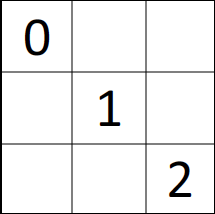
\includegraphics[scale=0.25]{sudoku-3.png}
\caption{Example of partial Latin Square of order 3.}
\end{figure}

\begin{figure}[H]
\label{fig:partialNP}
\centering
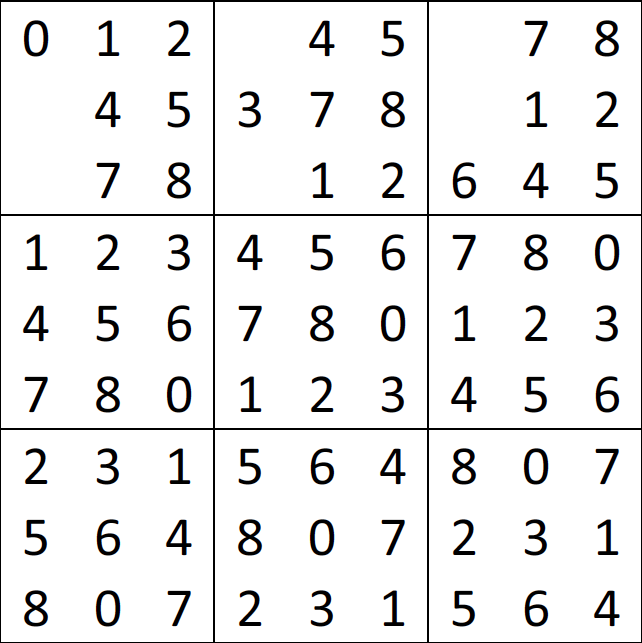
\includegraphics[scale=0.25]{sudoku-1.png}
\caption{Example of corresponding partial Number Place on a board of order 3.}
\end{figure}

\end{proof}

\section{Relationship to Other Complexity Classes.}
\label{sec:relationship}

In this section, we consider how $\mathsf{FCP}$ fits in relation to the well-known complexity classes, $\mathsf{NP}, \mathsf{coNP}, \mathsf{NP}^\mathsf{NP}, \mathsf{PSPACE}$. Recall that $\mathsf{NP}^\mathsf{NP}$ refers to the class of problems solvable in nondeterministic polynomial time with an $\mathsf{NP}$-oracle. We give a number of different containments, but it remains to be shown if any of these containments are strict.

\begin{proposition}
$\NP \subset \mathsf{FCP}$
\end{proposition}

\begin{proof}
If a problem is in $\NP$, then there exists an NTM which decides in time at most $p(n)$, where $p$ is a polynomial and $n$ is the size of the input. Thus, we can solve any problem in $\NP$ with the following equivalent $\mathsf{FCP}$ question: is there a partial (possibly full) certificate of size at most $p(n)$?
\end{proof}

\begin{corollary}
If a problem is $\mathsf{FCP}$-hard, it is also $\NP$-hard.
\end{corollary}

\begin{proposition}
If a problem is $\mathsf{FCP}$-hard, it is also $\coNP$-hard. 
\end{proposition}

\begin{proof}
Consider the problem of $\mathsf{UNIQUE-SAT}$, which gives a Boolean formula and asks if there is exactly one solution. This problem is known to be $\coNP$-hard \cite{blass1982unique}. We can solve $\mathsf{UNIQUE-SAT}$ by asking the following $\mathsf{FCP}$ question: given a Boolean formula, is there a partial certificate of size at most 0? If and only if such a certificate exists, then by definition of the Boolean formula is uniquely satisfiable.
\end{proof}

We switch our focus now to the problem of $\mathsf{FCP}$ SAT, an $\mathsf{FCP}$-complete problem. 

\begin{proposition}
$\mathsf{FCP}$ is contained in $\NP^{\NP}$.
\end{proposition}

\begin{proof}
We do this by providing an algorithm that solves $\mathsf{FCP}$ SAT with an NTM with a SAT oracle. 

The algorithm we give will rely on the following observations.

\textbf{Observation 1:} A Boolean formula $\phi$ has a partial assignment of $k$ variables which yield a unique solution if and only if for every variable outside the partial assignment, one assignment of this variable yields a satisfiable formula, and the other does not. This observation holds due to the fact that there is only one accepting branch.

\textbf{Observation 2:} A Boolean formula $\phi$ with a partial assignment of $k$ variables is \emph{not} uniquely satisfiable if and only if there exists a variable outside of the partial assignment for which both truth assignments of this variable give a satisfiable Boolean formula. This observation holds because this situation corresponds exactly with cases where we are not on a unique accepting branch.

To complete the proof, we simply give the algorithm:

\begin{codebox}
\Procname{$\mathsf{FCP}$ SAT: Instance: $\phi$ formula with variables $\{ x_i \}$ and variable $k$.}
\li \For $i = 1, ..., k$ \Then
\li Non-deterministically pick a variable $x_i$, without repetition
\li Non-deterministically pick an assignment \End
\li Iterate through all remaining variables \Then
\li \If a variable is such that both assignments give a satisfiable formula \Then
\li reject
\li \Else assign that variable \End \End
\li Once you have assigned all variables, accept.
\end{codebox}
\end{proof}


\section{Conclusion}
\label{sec:conclusion}

We have formalized the notion of what it means for a problem to be uniquely solvable after giving the fewest possible number of clues. This gave rise to the $\mathsf{FCP}$ class. We presented $\mathsf{FPC}$ versions of some classical $\NP$ problems and showed they were complete for this class. In particular, this means $\mathsf{FCP}$ Sudoku is $\NP$-hard, but is unlikely to be $\PSPACE$-hard. However, the instances of $\mathsf{FCP}$ Sudoku which make it $\mathsf{FCP}$-complete are very far from empty. In fact, just by looking at the last reduction from $\mathsf{FCP}$ Latin Squares, a Sudoku of dimensions $n^2 \times n^2$ which is a hard instance, at most $n^2$ of the $n^4$ squares at empty. It would be interesting to see if the empty instances of Sudoku are still complete for $\mathsf{FCP}$. This would be exactly the problem \cite{mcguire2012there} solved for $n = 3$. 

Further work in the field includes looking at other related results and adapting our framework to a the more general setting. The authors also think that it is important to determine where this class fits in the complexity zoo. In particular, there seem to be connections with the class $\#P$. A stricter notion of a reduction might also be required. Finally, it would be interesting to find problems in $\P$ such that their $\mathsf{SPC}$ versions are as hard for the class, or $\NP$-hard problems such that their $\mathsf{SPC}$ versions are not hard for the class. 

\bibliography{references}
\bibliographystyle{splncs}
\end{document}
